\documentclass{standalone}
\usepackage[T1]{fontenc}
\usepackage[latin2]{inputenc}
\usepackage[english]{babel}
\usepackage{tikz}
\usepackage{times}
\usetikzlibrary{calc,through,backgrounds,positioning,fit}
\usetikzlibrary{shapes,arrows,shadows}
 
\begin{document}
 
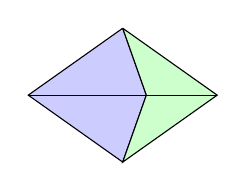
\begin{tikzpicture}[scale=1,inner sep=0.4mm]

\coordinate (p1) at (0,0); %dol
\coordinate (p2) at (0,1.7); %gora 
\coordinate (p3) at (-1.2,0.85); %dlugosc lewo
\coordinate (p4) at (1.2,0.85); %dlugosc prawo
\coordinate (p5) at (0.3,0.85); %srodek w prawo



\draw [fill=blue!20!] (p2) -- (p5) -- (p1) -- (p3) -- (p2);
\draw [fill=green!20!] (p2) -- (p5) -- (p1) -- (p4) -- (p2);
\draw (p3) -- (p4);
\end{tikzpicture}
 
\end{document}